This layer focuses on the systems needed to electronically propel the board and the systems needed to turn while in autonomous mode. The Jetson TX2 will be providing commands to an electronic speed controller to drive two brushless DC motors embedded into the rear truck. The front truck will be mounted onto a geared turning mechanism which will be rotated by a matching bevel gear using a stepper motor. The turning mechanism will be kept in place by two solenoids. To ensure that the turning mechanism is locked, the solenoid plunger will be monitored by an optical sensor. A micro-controller will be used to control the commutation of the motor, to engage the solenoids and to monitor the optical sensor.

\begin{figure}[h!]
	\centering
 	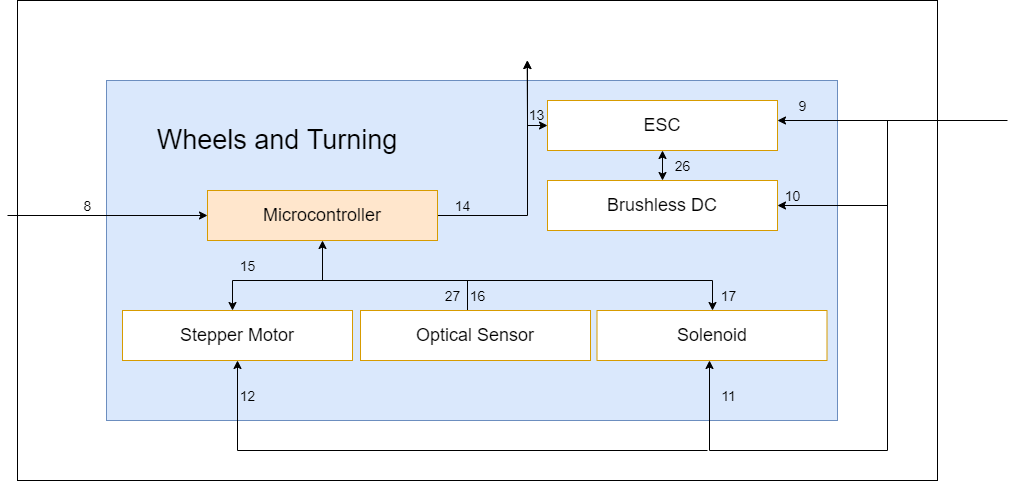
\includegraphics[width=0.60\textwidth]{images/Keaton/MicroC.png}
 \caption{Micro-Controller Subsystem in Wheels and Turning Layer}
\end{figure}

\subsection{Layer Hardware}
A Tiva TM4C123GH6PM micro-controller is used to manage lower level systems like the stepper motor, solenoids and optical sensors. This component is also used by the HMI and main control layer.

\subsection{Layer Operating System}
A custom Real Time Operating System (RTOS) developed for this project.

\subsection{Layer Software Dependencies}
The majority of software libraries were created internally for use with this project. Clock library sets the micro-controller to operate with a 16MHz crystal at a clock speed of 40MHz. GPIO library provides back-end register handling to control general purpose input and output pins. Shell library provides the ability for user input and instruction handling. UART0 library provides the ability to communicate with the micro-controller using the on-board USB port. Uartcom library is used for serial communication between the micro-controller and the Jetson TX2. Wait library provides a function to wait microseconds. Helperfunctions is a library used for parsing and other back-end functions. Kernel library is used for memory protection.

\subsection{Electronic Speed Controller}
The Electronic Speed Controller (ESC) is a hardware component that regulates the three-phase current to the brushless DC motors embedded in the rear truck.

%%%%%%%%%%%%%%%%%%%%%%%%%%%%%%%%%%%%%%%%%%%%%%%%%%%%%%%%%%
%  BE SURE TO UPDATE THE IMAGE CAPTION
\begin{figure}[h!]
	\centering
 	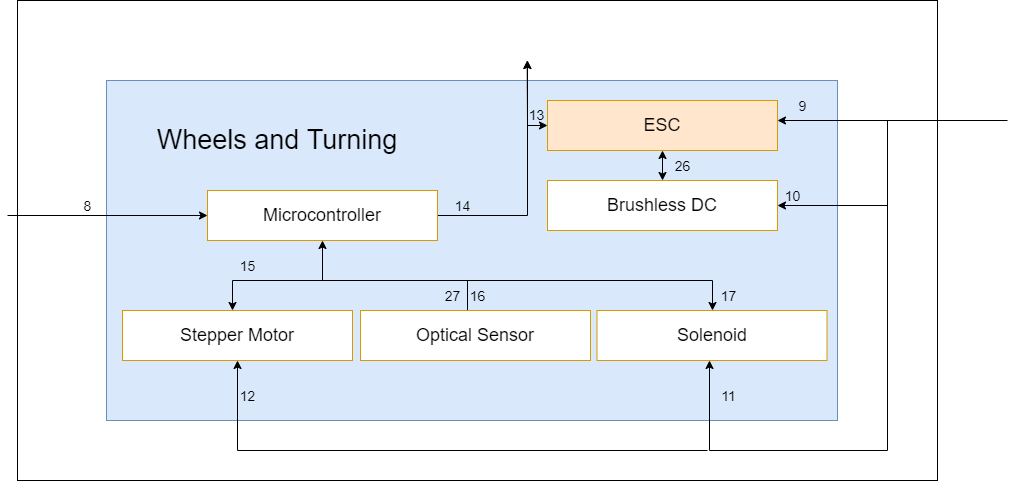
\includegraphics[width=0.60\textwidth]{images/Keaton/ESC.png}
 \caption{ESC Subsystem in Wheels and Turning Layer}
\end{figure}

\subsubsection{Subsystem Hardware}
The ESC is a hardware component that consists of two independent ESCs connected through a CAN bus. One ESC acts as the subordinate and mirrors everything programmed on the main, allowing both wheels to turn simultaneously.

\subsubsection{Subsystem Operating System}
The VESC Project firmware version 5.03.

\subsubsection{Subsystem Software Dependencies}
The Jetson TX2 is responsible for sending commands directly to the ESC through serial communication. A library created for the ESC is used.

\subsubsection{Subsystem Programming Languages}
Python to receive commands from the Jetson TX2. No Python running on the ESC.

\subsubsection{Subsystem Data Structures}
The data structure used in the ESC library is proprietary and belongs to the VESC project. 

\subsubsection{Subsystem Data Processing}
N/A

\subsection{Brushless DC Motors}
There are two brushless DC motors embedded in the rear truck of the long board. Each motor is six-hundred watts and receives its three-phase power from an electronic speed controller.

%%%%%%%%%%%%%%%%%%%%%%%%%%%%%%%%%%%%%%%%%%%%%%%%%%%%%%%%%%
%  BE SURE TO UPDATE THE IMAGE CAPTION
\begin{figure}[h!]
	\centering
 	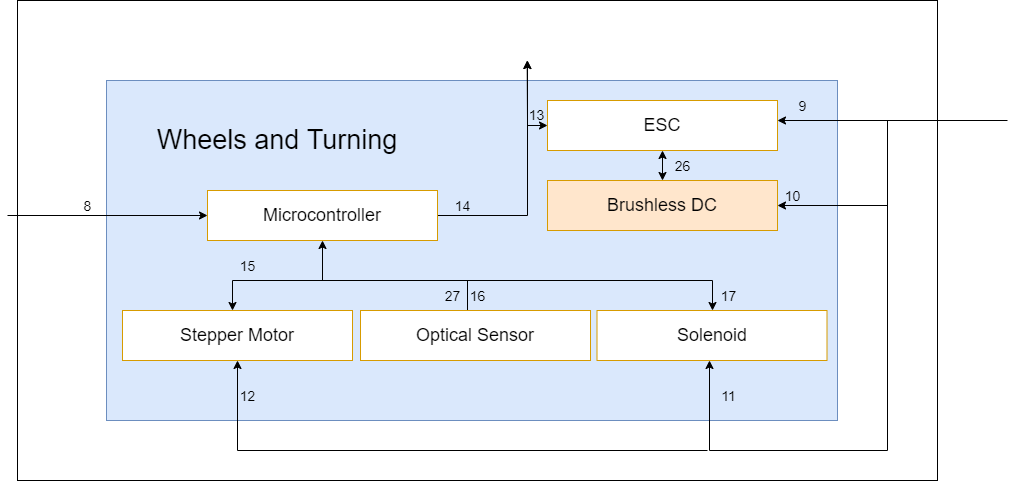
\includegraphics[width=0.60\textwidth]{images/Keaton/BLDC.png}
 \caption{BLDC Subsystem in Wheels and Turning Layer}
\end{figure}

\subsubsection{Subsystem Hardware}
The Brushless Direct Current Motor (BLDC) is a hardware component that consists of two six-hundred watt motors embedded in the rear truck. Each motor has three power wires corresponding to the three phases needed to electrically commutate the BLDC motor.

\subsubsection{Subsystem Operating System}
N/A

\subsubsection{Subsystem Software Dependencies}
An electronic speed controller is needed to regulate the current going into the motor.

\subsubsection{Subsystem Programming Languages}
N/A

\subsubsection{Subsystem Data Structures}
N/A

\subsubsection{Subsystem Data Processing}
N/A

\subsection{Stepper Motor}
A stepper motor is mounted on the underside of the board to interact with the turning mechanism. A bevel gear on the stepper motor shaft is connected to a matching gear on the turning mechanism which allows the board to rotate up to thirty-five degrees left or right of center.

%%%%%%%%%%%%%%%%%%%%%%%%%%%%%%%%%%%%%%%%%%%%%%%%%%%%%%%%%%
%  BE SURE TO UPDATE THE IMAGE CAPTION
\begin{figure}[h!]
	\centering
 	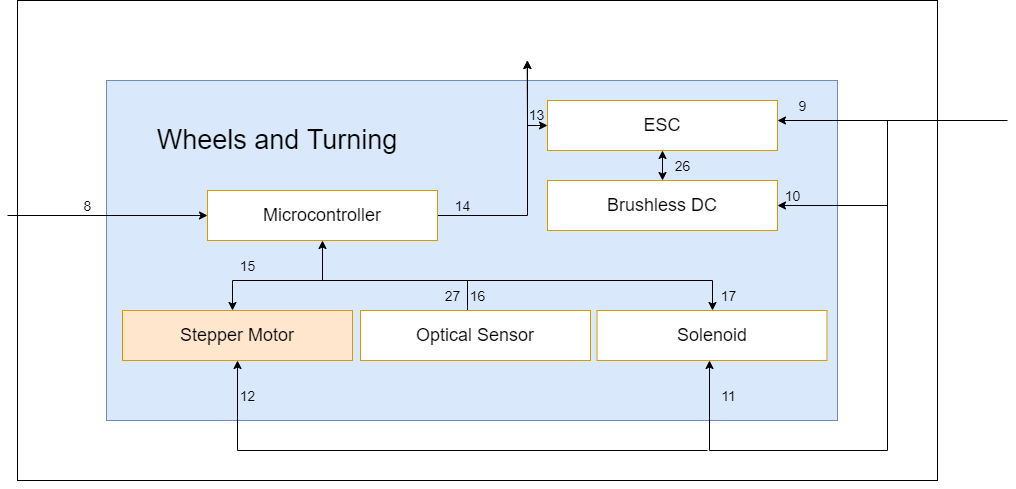
\includegraphics[width=0.60\textwidth]{images/Keaton/Stepper.png}
 \caption{Stepper Motor Subsystem in Wheels and Turning Layer}
\end{figure}

\subsubsection{Subsystem Hardware}
The NEMA-17 stepper motor is a hardware component that is driven by a DRV8825 motor driver. The motor is wired in a four wire configuration that operates off of twelve volts.

\subsubsection{Subsystem Operating System}
N/A

\subsubsection{Subsystem Software Dependencies}
The micro-controller interacts with the DRV8825 motor driver to commutate the motor in the chosen direction. A stepper motor library has been created to use with the RTOS code on the micro-controller.

\subsubsection{Subsystem Programming Languages}
C is used for the stepper motor library that is being run on the micro-controller.

\subsubsection{Subsystem Data Structures}
The DRV8825 steps the motor on the rising edge of a square wave. The time between steps varies depending on the speed needed for the turning mechanism. Direction of the motor is controlled by applying a high or low signal to the DIR pin. The motor changes direction upon a change in state of the DIR pin. No other data structures are needed to control the stepper motor.

\subsubsection{Subsystem Data Processing}
N/A

\subsection{Solenoid}
A solenoid is used to secure the turning mechanism so that the wheels are oriented in their neutral position. Applying power to the solenoid will pull the plunger out of the turning mechanism, allowing it to freely rotate as needed.

%%%%%%%%%%%%%%%%%%%%%%%%%%%%%%%%%%%%%%%%%%%%%%%%%%%%%%%%%%
%  BE SURE TO UPDATE THE IMAGE CAPTION
\begin{figure}[h!]
	\centering
 	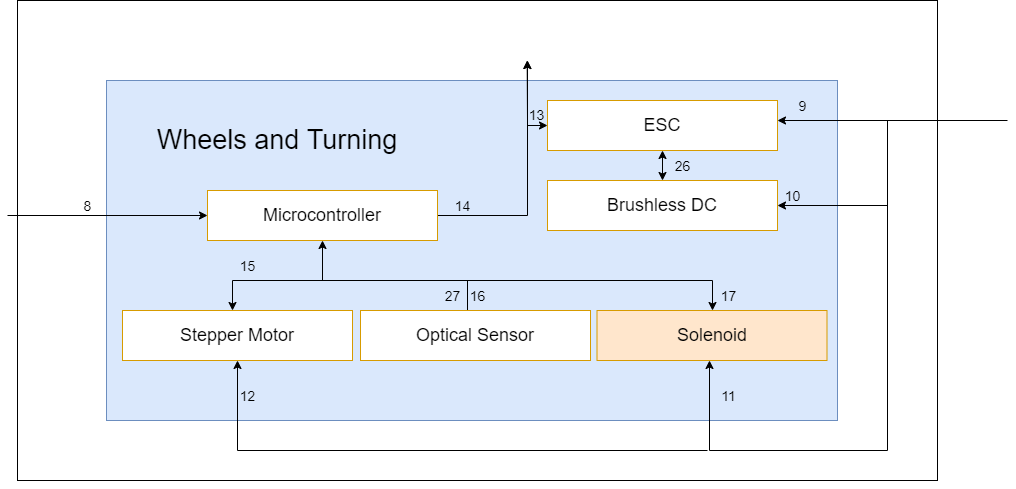
\includegraphics[width=0.60\textwidth]{images/Keaton/Solenoid.png}
 \caption{Solenoid Subsystem in Wheels and Turning Layer}
\end{figure}

\subsubsection{Subsystem Hardware}
The two solenoids are powered with 12V. A MOSFET will be configured to act as a switch, allowing power to flow through the solenoid.

\subsubsection{Subsystem Operating System}
N/A

\subsubsection{Subsystem Software Dependencies}
The micro-controller interacts with the MOSFET switch circuit, allowing the low current GPIO pins to determine if the solenoid is engaged or not. A solenoid library has been created to use with the RTOS code on the micro-controller.

\subsubsection{Subsystem Programming Languages}
C is used for the solenoid motor library that is being run on the micro-controller.

\subsubsection{Subsystem Data Structures}
With a MOSFET, the only data structure is toggling the GPIO pin on or off. This will engage or disengage the solenoid by allowing power to flow and cause the plunger to retract from the turning mechanism.

\subsubsection{Subsystem Data Processing}
N/A

\subsection{Optical Sensor}
An optical sensor will be used to determine if a solenoid has been fully engaged. When the solenoid has power applied, a plunger will be pulled out of the turning mechanism and the displaced shaft length will present at the rear of the solenoid. The optical sensor will be placed so that while engaged, the plunger at the back of the solenoid will break the optical beam of the sensor.

%%%%%%%%%%%%%%%%%%%%%%%%%%%%%%%%%%%%%%%%%%%%%%%%%%%%%%%%%%
%  BE SURE TO UPDATE THE IMAGE CAPTION
\begin{figure}[h!]
	\centering
 	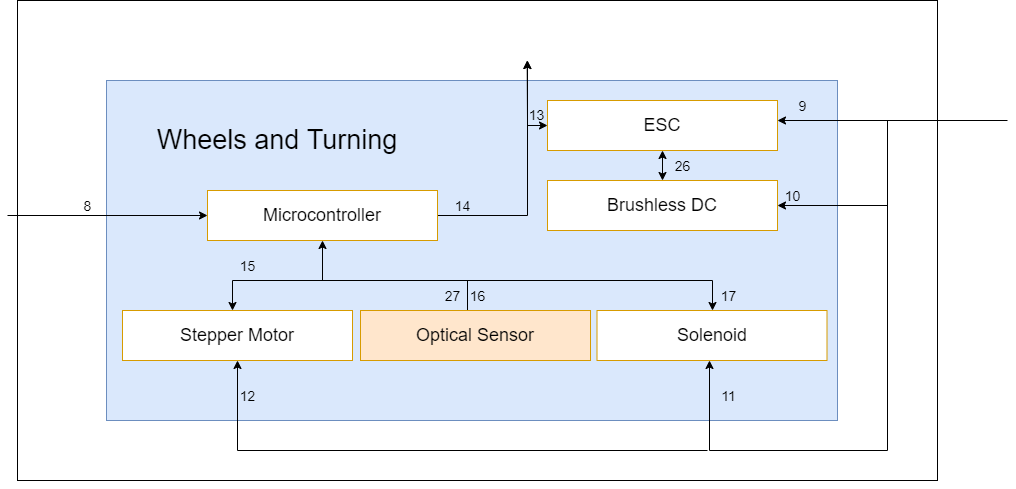
\includegraphics[width=0.60\textwidth]{images/Keaton/optical.png}
 \caption{Optical Subsystem in Wheels and Turning Layer}
\end{figure}

\subsubsection{Subsystem Hardware}
Two optical sensors wired between ground and a GPIO input pin.

\subsubsection{Subsystem Operating System}
N/A

\subsubsection{Subsystem Software Dependencies}
An optical sensor library has been created to use with the RTOS code on the micro-controller.

\subsubsection{Subsystem Programming Languages}
C is used for the optical sensor library that is being run on the micro-controller.

\subsubsection{Subsystem Data Structures}
The optical sensor is an input and will be constantly polled to ensure that the solenoid is in the correct position.

\subsubsection{Subsystem Data Processing}
N/A
